\documentclass[
    12pt, % Default font size, values between 10pt-12pt are allowed
    %spanish, % Uncomment for Spanish
]{fphw}

% Template-specific packages
\usepackage[utf8]{inputenc} % Required for inputting international characters
\usepackage[T1]{fontenc} % Output font encoding for international characters
\usepackage{fontspec,unicode-math} % Required for using utf8 characters in math mode
\usepackage{parskip}  % To add extra space between paragraphs
% \usepackage{mathpazo} % Use the Palatino font
\usepackage{graphicx} % Required for including images
\usepackage{booktabs} % Better horizontal rules in tables
\usepackage{hyperref} % For links (both internal and external)
\usepackage{listings} % Required for insertion of code
\usepackage{enumerate}% To modify the enumerate environment
\usepackage{cleveref} % Better \ref command -> \cref
\usepackage{import}   % This 4 packages and the command allow importing pdf
\usepackage{xifthen}  % figures generated with inkscape
\usepackage{pdfpages} % Source: https://castel.dev/post/lecture-notes-2/
\usepackage{mathtools}% Mathematical environments
\usepackage{relsize}  % \smaller and \mathsmaller commands
\usepackage{physics}  % A lot of good commands for mathematics
\usepackage[binary-units]{siunitx}  % To write magnitudes with units
\usepackage{transparent}
\newcommand{\incfig}[1]{%
    \def\svgwidth{0.95\columnwidth}
    \small
        \import{./images/}{#1.pdf_tex}
}

\setlength{\parindent}{15pt}
\setlength{\headheight}{22.8pt}

%----------------------------------------------------------------------------------------
%    ASSIGNMENT INFORMATION
%----------------------------------------------------------------------------------------

\title{Assignment 3 \\
    Parallelizing, Vectorizing and Optimizing the Memory Access
    of a Numerical Application} % Assignment title

\author{Emilio Domínguez Sánchez} % Student name

\date{December 27th, 2020} % Due date

\institute{University of Murcia \\ Faculty of Informatics} % Institute or school name

\class{Arquitectura y Organización de Computadores} % Course or class name

\professor{Dr. José Manuel García Carrasco} % Professor or teacher in charge of the assignment

%----------------------------------------------------------------------------------------
%    Definitions
%----------------------------------------------------------------------------------------

\lstset{
    language=C++,
    basicstyle=\footnotesize,        % the size of the fonts that are used for the code
    frame=L,
    captionpos=t,
    numbers=left,
    numbersep=10pt,
    breaklines=true,
    stepnumber=1,
    escapeinside={/*}{*/},
    showlines=true,
}
\newcommand{\tech}{\texttt}
\newcommand{\mtech}[1]{\text{\texttt{#1}}}
\newcommand{\gcc}{\textit{gcc}}
\newcommand{\clang}{\textit{clang}}
\newcommand{\icpc}{\textit{icpc}}
\newcommand{\OpenMp}{\textit{OpenMp}}

\begin{document}

\maketitle % Output the assignment title, created automatically using the information in the custom commands above

%----------------------------------------------------------------------------------------
%    ASSIGNMENT CONTENT
%----------------------------------------------------------------------------------------

\section*{Instructions for the student}

    In the resources folder there is an implementation of a micro-kernel that
solves the \textit{polar to cartesian binning problem}:
Given the polar coordinates of $n$ particles,
it is necessary to group them in equi-spaced rectangular bins
aligned with respect to cartesian coordinates.

\begin{enumerate}
    \item Parallelize the micro-kernel using \OpenMp{}.
    Include and discuss the \textit{speed up} obtained.

    \item Perform transformations to the code in order to
    allow the compiler's autovectorization.
    You may use the vectorization report of your compiler to detect the current problems.

    \item Optimize the memory access of the application.
    Study whether the techniques \textit{caché blocking} and \textit{unroll-and-jam}
    can be applied.

    \item Study how the accelerations that you have obtained vary according to
    the size of the problem (the number of particles and the number of bins).
\end{enumerate}
    
    You are also asked to write a document where you
explain breefly the positive aspects of the assignment,
as well as the negatives and
anything that you may have missed in it.

\newpage

%----------------------------------------------------------------------------------------

\section{Overview of the Original Code}

    The micro-kernel is a simple C++ function taking the radius and the angle of
a list of points and returning a the number of particles contained in each bin
(\cref{lst:original-micro-kernel}).
The output data is represented as a bidimensional array while
the input data is packed as an \textit{structure of arrays} (SoA)
(\cref{lst:original-defs}).
An \textit{structure of arrays} is a way of packing the data where
each field of a collection of structures is stored independently,
usually using an array of the type of that field.
Thus, the same field of contiguous elements of the collection
appear contiguously in memory,
allowing better vector optimizations when we need to operate
on the same field over consecutive elements.
In contrast, the traditional way of storing structures in most applications
is called \textit{array of structures} (AoS).

\begin{lstlisting}[
    caption=Micro-Kernel,
    gobble=4,
    label=lst:original-micro-kernel,
]
    void BinParticles(const InputDataType& inputData, BinsType& outputBins) {
      for (int i = 0; i < inputData.numDataPoints; i++) { 
        // Transforming from cylindrical to Cartesian coordinates:
        const FTYPE x = inputData.r[i]*COS(inputData.phi[i]);
        const FTYPE y = inputData.r[i]*SIN(inputData.phi[i]);

        // Calculating the bin numbers for these coordinates:
        const int iX = int((x - xMin)*binsPerUnitX);
        const int iY = int((y - yMin)*binsPerUnitY);

        // Incrementing the appropriate bin in the counter
        ++outputBins[iX][iY];
      }
    }

\end{lstlisting}

    The code is conceptually simple, we need to apply the transformation
\begin{equation*}
    (r, \phi) \mapsto r(\cos{\phi}, \sin{\phi}) \eqqcolon (x, y)
\end{equation*}
%
to each particle,
and add $1$ to the bin where this particle is located.
There are $\mtech{nBinsX} \times \mtech{nBinsY}$
covering the range where the particles may lay,
$[\mtech{xMin}, \mtech{xMax}] \times [\mtech{yMin}, \mtech{yMax}]$.
That gives each bin the size
$\frac{1}{\mtech{binsPerUnitX}} \times \frac{1}{\mtech{binsPerUnitY}}$\footnote{
    In general, we would have computed the size as a pair of values $w \times h$
    and written a division in the code because it is more natural.
    But division is a slow operation.
    Thus, we compute $\frac{1}{w}$ and $\frac{1}{h}$ instead.
}.

\begin{lstlisting}[
    caption=Main definitions of the original code,
    gobble=4,
    label=lst:original-defs,
]
    #ifdef DOUBLE_PRECISION
    #define FTYPE double
    #define SIN sin
    #define COS cos
    #else
    #define FTYPE float
    #define SIN sinf
    #define COS cosf
    #endif

    // Input data arrives as arrays of cylindrical coordinates
    // of particles: r and phi. Size of each array is numDataPoints
    struct InputDataType {
      int numDataPoints;
      FTYPE* r;
      FTYPE* phi;
    };


    // The application bins particles defined in InputDataType
    // into bins in Cartesian coordinates
    const int nBinsX=10;
    const int nBinsY=10;
    typedef int BinsType[nBinsX][nBinsY];

    // We assume that the radial coordinate does not exceed this value
    const FTYPE maxMagnitudeR=5.0;

    // Boundaries of bins:
    const FTYPE xMin = -maxMagnitudeR*1.000001;
    const FTYPE xMax = +maxMagnitudeR*1.000001;
    const FTYPE yMin = -maxMagnitudeR*1.000001;
    const FTYPE yMax = +maxMagnitudeR*1.000001;

    // Reciprocal of widths of bins:
    const FTYPE binsPerUnitX = (FTYPE)nBinsX/(xMax - xMin);
    const FTYPE binsPerUnitY = (FTYPE)nBinsY/(yMax - yMin);

\end{lstlisting}

\section{Extra: Making use of C++ features and modern cross compiler solutions}

    The micro-kernel given to us was a C++ application but the code looked more like C.
In addition, some of the techniques studied in class to perform the transformations
are seen for a specific compiler.
Modern C and C++ include directives that allow to work with aligned types.
This makes it possible to write code that is simpler and cross-compiler.

\begin{figure}[h]
    \centering
    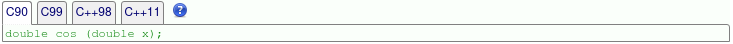
\includegraphics[width=0.95\textwidth]{prac3/media/cos_c90_reference.png}
    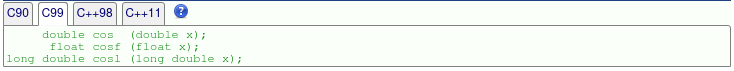
\includegraphics[width=0.95\textwidth]{prac3/media/cos_c99_reference.png}
    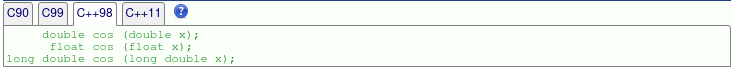
\includegraphics[width=0.95\textwidth]{prac3/media/cos_cpp98_reference.png}
    \caption{Documentation for the \tech{cos} function in C and C++
    taken from \url{https://www.cplusplus.com/reference/cmath/cos/}}
\end{figure}

    For instance, the code is using its own macros to
call different trigonometric functions depending on the data types
(\cref{lst:trigonometric-defines}).
In general, this should be achieved using language features such as function overloading.
The usage comes from the fact that C90 did not provide this overloads,
even though C99 does.

\begin{lstlisting}[gobble=4, label=lst:trigonometric-defines]
    #ifdef DOUBLE_PRECISION
    #define FTYPE double
    #define SIN sin
    #define COS cos
    #else
    #define FTYPE float
    #define SIN sinf
    #define COS cosf
    #endif
    /*[$\ldots$]*/
    const FTYPE x = inputData.r[i]*COS(inputData.phi[i]);
    const FTYPE y = inputData.r[i]*SIN(inputData.phi[i]);

\end{lstlisting}

    But because the code is C++ and it is not even convertible to C as is
(even the micro-kernel function uses references),
it is natural to use the function overloading,
as it was already provided in the oldest standard of C++ (C++98).

\begin{lstlisting}[gobble=4]
    const FTYPE x = inputData.r[i]*std::cos(inputData.phi[i]);
    const FTYPE y = inputData.r[i]*std::sin(inputData.phi[i]);

\end{lstlisting}

    More problematic is the usage of compiler specific options.
Sometimes they are needed, but for the pourposes of alignment,
we already have solutions builtin to the newer versions of the language.
For the old versions,
it is better to stick to alternatives which are supported by multiple compilers.

\begin{table}[h]
    \centering
    \begin{tabular}{m{0.22\textwidth} c m{0.32\textwidth}}
        \textbf{Task} &
            \textbf{Intel ICPC Specific Solution} &
                \textbf{Language Feature} \\
        \hline \\

        Declaring and querying align requirements for types or objects. &
            attributes &
                keywords \tech{alignas} and \tech{alignof} (since C++11) \\[2em]
        Reserving and freeing aligned memory. &
            \tech{\_\_mm\_malloc} and \tech{\_\_mm\_free} &
                \tech{std::aligned\_alloc} or automatic with \tech{operator new}
                (since C++17) \\[2em]
        Hinting the compiler about the alignment of a pointer. &
            \tech{\#pragma vector aligned} &
                \tech{std::assume\_aligned} (since C++20) \\[2em]
    \end{tabular}
    \caption{C++ handling of alignment requirements}
\end{table}

    The code can benefit greatly from the use of some C++ constructs.
For example, the use of constexpr variables ensures
the compiler knows some values in advance.
How does this apply?
In the code, for example, we are multiplying by the reciprocal instead of dividing.
When that value is known in compile time, which we now can assure,
the compiler can easily transform a division into a multiplication,
and there is no need to change our code.
Even though this does not apply when that value is not known at compile time,
it is very useful.
Another benefit is using type aliases instead of defines
(although this could already be done in plain C).

\begin{lstlisting}[
    gobble=4,
    caption=Some of the changes applied to the code,
]
    < #ifdef DOUBLE_PRECISION
    < #define FTYPE double
    < #define SIN sin
    < #define COS cos
    < #else
    < #define FTYPE float
    < #define SIN sinf
    < #define COS cosf
    ---
    > #ifdef DOUBLE_PRECISION
    > using FTYPE = double;
    > #else
    > using FTYPE = float;
    35c29,31
    < typedef int BinsType[nBinsX][nBinsY];
    ---
    > using BinsType = int[nBinsX][nBinsY];
    38c34
    < const FTYPE maxMagnitudeR=5.0;
    ---
    > constexpr FTYPE maxMagnitudeR = 5.0;
    > void BinParticlesReference(const InputDataType& inputData, BinsType& outputBins) {
    63,64c59,60
    <     const FTYPE x = inputData.r[i]*COS(inputData.phi[i]);
    <     const FTYPE y = inputData.r[i]*SIN(inputData.phi[i]);
    ---
    >     const FTYPE x = inputData.r[i]*std::cos(inputData.phi[i]);
    >     const FTYPE y = inputData.r[i]*std::sin(inputData.phi[i]);
    67,68c63,64
    <     const int iX = int((x - xMin)*binsPerUnitX);
    <     const int iY = int((y - yMin)*binsPerUnitY);
    ---
    >     const size_t iX = (x - xMin)*binsPerUnitX;
    >     const size_t iY = (y - yMin)*binsPerUnitY;
    81c77,80
    <       if (fabs(binnedData[i][j] - binnedDataRef[i][j]) > 1e-5*(binnedData[i][j] + binnedDataRef[i][j])) {
    ---
    >       if (std::abs(binnedData[i][j] - binnedDataRef[i][j]) > 1e-5*(binnedData[i][j] + binnedDataRef[i][j])) {

\end{lstlisting}

\section{Parallelization}

\begin{lstlisting}[
    gobble=4,
    label=lst:parallelization,
    caption=Parallelization of the code using \OpenMp{},
]
    void BinParticles(const InputDataType& inputData, BinsType& outputBins) {
      #pragma omp parallel for reduction(+:outputBins)
      for (int i = 0; i < inputData.numDataPoints; i++) { 
        // Transforming from cylindrical to Cartesian coordinates:
        const FTYPE x = inputData.r[i]*std::cos(inputData.phi[i]);
        const FTYPE y = inputData.r[i]*std::sin(inputData.phi[i]);

        // Calculating the bin numbers for these coordinates:
        const size_t iX = (x - xMin)*binsPerUnitX;
        const size_t iY = (y - yMin)*binsPerUnitY;

        // Incrementing the appropriate bin in the counter
        ++outputBins[iX][iY];
      }
    }

\end{lstlisting}

    Parallelizing the micro-kernel as is should be straight forward.
The only shared data between iterations of the loop is the \tech{outputBins} variable.
And that variable is accessed using the coordinates \tech{iX} and \tech{iY}
which are dependent on the data.
Hence, the access to the shared memory is random and can be conflicting.
The best solution to this problem is applying a reduction over \tech{outputBins},
as seen in \cref{lst:parallelization}.

\subsection{Execution Environment}

    I tried the executing the codes with \gcc{}, \clang{} and \icpc{}.
It was not possible to execute the codes that are yet to come with \gcc{} or \clang{}
because they could not vectorize it.
Therefore, all of the results shown are compiling with \icpc{}.

\subsection{Execution Results}

\begin{lstlisting}[
    gobble=4,
    caption=Execution results after parallelization.
    The speed up is close to the number of cores.,
]
    Particle Binning Optimization Demo (single precision)
    Additional information is available in accompanying papers at http://colfaxresearch.com/

    (c) Colfax International, 2015.

    Initialization... done in 1.286 seconds.
    Computing reference result... done in 0.794 seconds.
    Baseline performance:   8.45e-02 GP/s

    Benchmarking...

      Trial    Time, s    Speedup       GP/s *
          1  2.146e-01       3.70   3.13e-01 **
          2  2.145e-01       3.70   3.13e-01 **
          3  2.141e-01       3.71   3.13e-01 
          4  2.142e-01       3.71   3.13e-01 
          5  2.145e-01       3.70   3.13e-01 
          6  2.141e-01       3.71   3.13e-01 
          7  2.141e-01       3.71   3.13e-01 
          8  2.145e-01       3.70   3.13e-01 
          9  2.141e-01       3.71   3.13e-01 
         10  2.144e-01       3.70   3.13e-01 
    ---------------------------------------------------------
    Optimized performance:   3.71   3.13e-01 +- 2.47e-04 GP/s
    ---------------------------------------------------------
    *  - Performance unit 1 GP/s is 10^9 particles binned per second.
    ** - warm-up, not included in average

\end{lstlisting}

\section{Vectorization}

    The vectorization is harder than the parallelization in this particular case
because it requires better understanding of the code execution.
We are accessing the array \tech{outputBins} non linearly.
However, most of the work,
the cosine and sine functions\footnote{
    Behind a simple mathematical function call we can encounter
    a highly optimized taylor expansion, for instance.
}, is done before that and is vectorizable.
The trick here is to split the loop.
In a first loop we will calculate the transformed coordinates
and in a second loop we will modify the array \tech{outputBins}.
Nonetheless, if our vector size is $4$ or $8$,
the speed up will be less because only one part of the code is being vectorized,
but we hope that it is big enough.

    Vectorization also requires that the data is aligned in memory\footnote{
    For very large input the compiler usually strips
    a portion from the beginning and from the end of the array
    during run time and performs aligned operations on the remaining part.
    For small arrays, this can take a considerable amount of relative time,
    but for big arrays this time is negligible.
    However, if we also want to parallelize, it is even harder for the compiler,
    because it needs to strip and then divide the remaining part among the threads.
}
Generally, to the size of the vector.
Actually, it is true that it is not a strict requirement for Intel compilers,
only that the code will otherwise execute slower.
Consequently, in order to execute SSE vector operations (\textit{fast}),
we need to align our data to a $16$ byte bounday,
while if we want to execute AVX2 vector operations,
we need to align our data to a $32$ byte boundary.

\begin{lstlisting}[
    gobble=4,
    label=lst:vectorization-with-alloc,
    caption=Vectorization of the code splitting the main loop,
]
    void BinParticles(const InputDataType& inputData, BinsType& outputBins) {
      constexpr int TILE_SIZE = 64;
      FTYPE* r = std::assume_aligned<ALIGNMENT>(inputData.r);
      FTYPE* phi = std::assume_aligned<ALIGNMENT>(inputData.phi);
      static int* iX = (int*) std::aligned_alloc(ALIGNMENT,
          sizeof(FTYPE)*inputData.numDataPoints);
      static int* iY = (int*) std::aligned_alloc(ALIGNMENT,
          sizeof(FTYPE)*inputData.numDataPoints);
      for (size_t ii = 0; ii < (size_t) inputData.numDataPoints; ii+=TILE_SIZE) {
        for (size_t i = 0; i < TILE_SIZE; i++) { 
          // Transforming from cylindrical to Cartesian coordinates:
          const FTYPE x = r[ii+i]*std::cos(phi[ii+i]);
          const FTYPE y = r[ii+i]*std::sin(phi[ii+i]);

          // Calculating the bin numbers for these coordinates:
          // const size_t iX = (x - xMin)*binsPerUnitX;
          // const size_t iY = (y - yMin)*binsPerUnitY;
          iX[i] = (x - xMin)*binsPerUnitX;
          iY[i] = (y - yMin)*binsPerUnitY;
        }
        for (size_t i = 0; i < TILE_SIZE; ++i) {
          // Incrementing the appropriate bin in the counter
          ++outputBins[iX[i]][iY[i]];
        }
      }
    }

\end{lstlisting}

    \Cref{lst:vectorization-with-alloc} shows the code
ready to be vectorized by the compiler\footnote{
    Note that in this code we are assuming that
    the vector size is multiple of \tech{TILE\_SIZE}.
    We would have to include another loop that handled the extra elements.
}. The function now needs to allocate on the heap,
because the vector is so big that it would not fit in the stack.
Reserving and freeing this array increases substantially the execution time.
A solution is reserving the memory once for all the function calls.
We can either convert the function into a functor which
reserves a maximum ammount of memory upon initialization or
reserve it in a global static variable at the beginning of the program.
The nicer alternative is to use a smaller array,
which we will discuss in the following section.

\subsection{Execution Results}

    In this case the speed up is a bit further from $8$, the size of a vector.
However, this is due to the fact that only a part of the work was parallelizable.
Luckily, it was a big part.

\begin{lstlisting}[
    gobble=4,
    caption={Execution results after vectorization.
    The speed up is close to 8, the size of a vector.},
]
    Particle Binning Optimization Demo (single precision)
    Additional information is available in accompanying papers at http://colfaxresearch.com/

    (c) Colfax International, 2015.

    Initialization... done in 1.221 seconds.
    Computing reference result... done in 0.794 seconds.
    Baseline performance:   8.45e-02 GP/s

    Benchmarking...

      Trial    Time, s    Speedup       GP/s *
          1  1.143e-01       6.95   5.87e-01 **
          2  1.145e-01       6.94   5.86e-01 **
          3  1.142e-01       6.95   5.88e-01 
          4  1.151e-01       6.90   5.83e-01 
          5  1.144e-01       6.94   5.86e-01 
          6  1.145e-01       6.94   5.86e-01 
          7  1.146e-01       6.93   5.85e-01 
          8  1.144e-01       6.94   5.86e-01 
          9  1.157e-01       6.86   5.80e-01 
         10  1.143e-01       6.95   5.87e-01 
    ---------------------------------------------------------
    Optimized performance:   6.93   5.85e-01 +- 2.39e-03 GP/s
    ---------------------------------------------------------
    *  - Performance unit 1 GP/s is 10^9 particles binned per second.
    ** - warm-up, not included in average

\end{lstlisting}

\section{Memory Access Optimization}

    The memory access optimizations known as \textit{tiling} are a set
of techniques that try to alter the patterns in which the memory is accessed
to group operations that act on the same memory.
This increases the performance of \textit{memory bound} applications because
it reduces the number of accesses to main memory.

    In our original program, it is impossible to improve the memory access pattern.
We access the variables \tech{inputData.r} and \tech{inputData.phi} sequentially.
Each piece of information is brought from memory, used and discarded
and is not used again.
The loop tiling techniques increase the performance because they erase the need
of retrieving the value from main memory once again to perform more operations.
However, if there is a single retrieval per value,
there is no room for improvement in that sense.
In addition, if the data is accessed sequentially,
the whole block brought from memory is useful and
the hardware prefetching works perfectly.
We also write to the variable \tech{outputBins},
but the access is completely random.

    However, the vectorized code can benefit from this techniques,
because in the vectorized code we are declaring an auxiliary array.
That is, we are storing information in main memory and then reading it.
Instead, we can work with chunks of data and use a smaller array,
one that fits in caché.
In the process, we also get rid of the extra allocations and the time they consumed.

We can also hint the compiler to unroll this loop
when we select a small \tech{TILE\_SIZE}.
Take into account that the vectorized loop can have $8$ times less iterations.
Therefore, a loop of $32$ iterations can be unrolled by copying the code just $4$ times.
This hint is usually not needed because
modern compiler are capable of deciding when unrolling is beneficial.

\begin{lstlisting}[
    gobble=4,
    label=lst:vectorization,
    caption=Tiled version of the vectorized code,
]
    void BinParticles(const InputDataType& inputData, BinsType& outputBins) {
      constexpr int TILE_SIZE = 64;
      FTYPE* r = std::assume_aligned<ALIGNMENT>(inputData.r);
      FTYPE* phi = std::assume_aligned<ALIGNMENT>(inputData.phi);
      int iX[TILE_SIZE];
      int iY[TILE_SIZE];
      for (size_t ii = 0; ii < (size_t) inputData.numDataPoints; ii+=TILE_SIZE) {
        for (size_t i = 0; i < TILE_SIZE; i++) { 
          // Transforming from cylindrical to Cartesian coordinates:
          const FTYPE x = r[ii+i]*std::cos(phi[ii+i]);
          const FTYPE y = r[ii+i]*std::sin(phi[ii+i]);

          // Calculating the bin numbers for these coordinates:
          iX[i] = (x - xMin)*binsPerUnitX;
          iY[i] = (y - yMin)*binsPerUnitY;
        }
        for (size_t i = 0; i < TILE_SIZE; ++i) {
          // Incrementing the appropriate bin in the counter
          ++outputBins[iX[i]][iY[i]];
        }
      }
    }

\end{lstlisting}

\subsection{Execution Results}

    We can see that the speed up is the same as with the vectorized code.
We can conclude we were not wasting extra time by using an auxiliary array.
However, there is also another big benefit and is the reduced memory needed.
Memory complexity is also important.
Furthermore, in the previous case we had a fast function
because we were relying of statically allocated memory.
Allocating during each call did also hurt the performance.

\begin{lstlisting}[
    gobble=4,
    caption=Execution results after vectorization with loop tiling.
    The speed up is similar to the untiled version.,
]
    Particle Binning Optimization Demo (single precision)
    Additional information is available in accompanying papers at http://colfaxresearch.com/

    (c) Colfax International, 2015.

    Initialization... done in 1.225 seconds.
    Computing reference result... done in 0.792 seconds.
    Baseline performance:   8.47e-02 GP/s

    Benchmarking...

      Trial    Time, s    Speedup       GP/s *
          1  1.159e-01       6.84   5.79e-01 **
          2  1.170e-01       6.77   5.74e-01 **
          3  1.161e-01       6.82   5.78e-01 
          4  1.163e-01       6.82   5.77e-01 
          5  1.162e-01       6.82   5.78e-01 
          6  1.161e-01       6.82   5.78e-01 
          7  1.171e-01       6.76   5.73e-01 
          8  1.160e-01       6.83   5.78e-01 
          9  1.159e-01       6.84   5.79e-01 
         10  1.158e-01       6.84   5.79e-01 
    ---------------------------------------------------------
    Optimized performance:   6.82   5.78e-01 +- 1.90e-03 GP/s
    ---------------------------------------------------------
    *  - Performance unit 1 GP/s is 10^9 particles binned per second.
    ** - warm-up, not included in average

\end{lstlisting}

\section{Global Speed Up}

    Our goal now is to combine all the techniques.
The last version of the code, \cref{lst:vectorization},
only lacks parallelism.

\begin{lstlisting}[
    gobble=4,
    label=lst:vectorization,
    caption=Fully optimized version of the micro-kernel,
]
    void BinParticles(const InputDataType& inputData, BinsType& outputBins) {
      constexpr int TILE_SIZE = 64;
      FTYPE* r = std::assume_aligned<ALIGNMENT>(inputData.r);
      FTYPE* phi = std::assume_aligned<ALIGNMENT>(inputData.phi);
      #pragma omp parallel reduction(+:outputBins)
      {
        // This variables need to be private to each thread
        int iX[TILE_SIZE];
        int iY[TILE_SIZE];
        #pragma omp for
        for (size_t ii = 0; ii < (size_t) inputData.numDataPoints; ii+=TILE_SIZE) {
          for (size_t i = 0; i < TILE_SIZE; i++) { 
            // Transforming from cylindrical to Cartesian coordinates:
            const FTYPE x = r[ii+i]*std::cos(phi[ii+i]);
            const FTYPE y = r[ii+i]*std::sin(phi[ii+i]);

            // Calculating the bin numbers for these coordinates:
            iX[i] = (x - xMin)*binsPerUnitX;
            iY[i] = (y - yMin)*binsPerUnitY;
          }
          for (size_t i = 0; i < TILE_SIZE; ++i) {
            // Incrementing the appropriate bin in the counter
            ++outputBins[iX[i]][iY[i]];
          }
        }
      }
    }

\end{lstlisting}

\subsection{Execution Results}

    Combining parallelization and vectorization we obtain a speed up of $24.84$,
very close to the product of the speed up of both methods, $6.93\cdot 3.71 = 25.71$.

\begin{lstlisting}[
    gobble=4,
    caption=Execution results after vectorization with loop tiling.
    The program ends up being almost $25$ times faster than the original.,
]
    Particle Binning Optimization Demo (single precision)
    Additional information is available in accompanying papers at http://colfaxresearch.com/

    (c) Colfax International, 2015.

    Initialization... done in 1.277 seconds.
    Computing reference result... done in 0.794 seconds.
    Baseline performance:   8.45e-02 GP/s

    Benchmarking...

      Trial    Time, s    Speedup       GP/s *
          1  3.227e-02      24.61   2.08e+00 **
          2  3.192e-02      24.88   2.10e+00 **
          3  3.198e-02      24.83   2.10e+00 
          4  3.199e-02      24.82   2.10e+00 
          5  3.202e-02      24.80   2.10e+00 
          6  3.192e-02      24.88   2.10e+00 
          7  3.196e-02      24.85   2.10e+00 
          8  3.195e-02      24.86   2.10e+00 
          9  3.202e-02      24.80   2.10e+00 
         10  3.195e-02      24.86   2.10e+00 
    ---------------------------------------------------------
    Optimized performance:  24.84   2.10e+00 +- 2.28e-03 GP/s
    ---------------------------------------------------------
    *  - Performance unit 1 GP/s is 10^9 particles binned per second.
    ** - warm-up, not included in average

\end{lstlisting}

\section{Performance Compared to Problem Size}

    We were asked to test the performance of the program
when increasing the size of the problem past $n = 2^{27}$ and
when reducing the number of bins to half.
The tests I carried don't show any difference in speedup.
What I would like to test now would be the speed up when
the size of the problem is small.
In those cases, the alignment is critical because stripping parts
from the beginning and end of a small vector to handle misalignment
takes, comparatively, more time.
Unfortunately, I lack a system where I can install and test the \icpc{} compiler freely.

%----------------------------------------------------------------------------------------

\end{document}
